% Created by tikzDevice version 0.12.6 on 2026-01-26 17:00:54
% !TEX encoding = UTF-8 Unicode
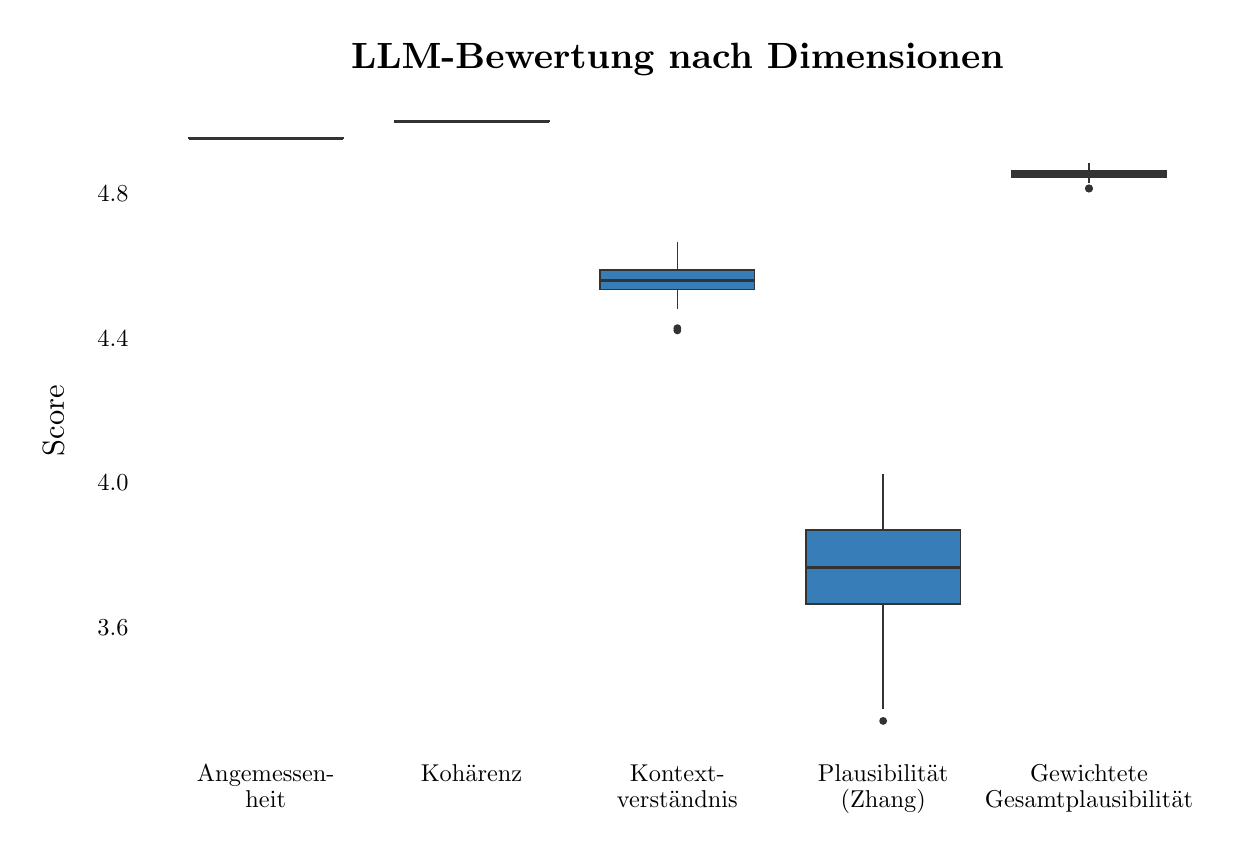
\begin{tikzpicture}[x=1pt,y=1pt]
\definecolor{fillColor}{RGB}{255,255,255}
\path[use as bounding box,fill=fillColor,fill opacity=0.00] (0,0) rectangle (433.62,289.08);
\begin{scope}
\path[clip] (  0.00,  0.00) rectangle (433.62,289.08);
\definecolor{fillColor}{RGB}{255,255,255}

\path[fill=fillColor] (  0.00,  0.00) rectangle (433.62,289.08);
\end{scope}
\begin{scope}
\path[clip] ( 41.41, 27.73) rectangle (428.12,266.40);
\definecolor{drawColor}{gray}{0.20}

\path[draw=drawColor,line width= 0.6pt,line join=round] ( 86.03,249.34) -- ( 86.03,249.34);

\path[draw=drawColor,line width= 0.6pt,line join=round] ( 86.03,249.18) -- ( 86.03,249.18);
\definecolor{fillColor}{RGB}{55,126,184}

\path[draw=drawColor,line width= 0.6pt,fill=fillColor] ( 58.14,249.34) --
	( 58.14,249.18) --
	(113.91,249.18) --
	(113.91,249.34) --
	( 58.14,249.34) --
	cycle;

\path[draw=drawColor,line width= 1.1pt] ( 58.14,249.18) -- (113.91,249.18);

\path[draw=drawColor,line width= 0.6pt,line join=round] (160.39,255.39) -- (160.39,255.56);

\path[draw=drawColor,line width= 0.6pt,line join=round] (160.39,255.23) -- (160.39,255.06);

\path[draw=drawColor,line width= 0.6pt,fill=fillColor] (132.51,255.39) --
	(132.51,255.23) --
	(188.28,255.23) --
	(188.28,255.39) --
	(132.51,255.39) --
	cycle;

\path[draw=drawColor,line width= 1.1pt] (132.51,255.23) -- (188.28,255.23);
\definecolor{fillColor}{gray}{0.20}

\path[draw=drawColor,line width= 0.4pt,line join=round,line cap=round,fill=fillColor] (234.76,179.69) circle (  1.21);

\path[draw=drawColor,line width= 0.4pt,line join=round,line cap=round,fill=fillColor] (234.76,180.50) circle (  1.21);

\path[draw=drawColor,line width= 0.6pt,line join=round] (234.76,201.47) -- (234.76,211.57);

\path[draw=drawColor,line width= 0.6pt,line join=round] (234.76,194.52) -- (234.76,187.37);
\definecolor{fillColor}{RGB}{55,126,184}

\path[draw=drawColor,line width= 0.6pt,fill=fillColor] (206.88,201.47) --
	(206.88,194.52) --
	(262.65,194.52) --
	(262.65,201.47) --
	(206.88,201.47) --
	cycle;

\path[draw=drawColor,line width= 1.1pt] (206.88,197.75) -- (262.65,197.75);
\definecolor{fillColor}{gray}{0.20}

\path[draw=drawColor,line width= 0.4pt,line join=round,line cap=round,fill=fillColor] (309.13, 38.57) circle (  1.21);

\path[draw=drawColor,line width= 0.6pt,line join=round] (309.13,107.49) -- (309.13,127.85);

\path[draw=drawColor,line width= 0.6pt,line join=round] (309.13, 80.76) -- (309.13, 42.99);
\definecolor{fillColor}{RGB}{55,126,184}

\path[draw=drawColor,line width= 0.6pt,fill=fillColor] (281.24,107.49) --
	(281.24, 80.76) --
	(337.02, 80.76) --
	(337.02,107.49) --
	(281.24,107.49) --
	cycle;

\path[draw=drawColor,line width= 1.1pt] (281.24, 94.01) -- (337.02, 94.01);
\definecolor{fillColor}{gray}{0.20}

\path[draw=drawColor,line width= 0.4pt,line join=round,line cap=round,fill=fillColor] (383.50,230.93) circle (  1.21);

\path[draw=drawColor,line width= 0.4pt,line join=round,line cap=round,fill=fillColor] (383.50,231.00) circle (  1.21);

\path[draw=drawColor,line width= 0.6pt,line join=round] (383.50,237.34) -- (383.50,240.32);

\path[draw=drawColor,line width= 0.6pt,line join=round] (383.50,235.19) -- (383.50,233.06);
\definecolor{fillColor}{RGB}{55,126,184}

\path[draw=drawColor,line width= 0.6pt,fill=fillColor] (355.61,237.34) --
	(355.61,235.19) --
	(411.39,235.19) --
	(411.39,237.34) --
	(355.61,237.34) --
	cycle;

\path[draw=drawColor,line width= 1.1pt] (355.61,236.20) -- (411.39,236.20);
\end{scope}
\begin{scope}
\path[clip] (  0.00,  0.00) rectangle (433.62,289.08);
\definecolor{drawColor}{RGB}{0,0,0}

\node[text=drawColor,anchor=base east,inner sep=0pt, outer sep=0pt, scale=  0.88] at ( 36.46, 69.39) {3.6};

\node[text=drawColor,anchor=base east,inner sep=0pt, outer sep=0pt, scale=  0.88] at ( 36.46,121.72) {4.0};

\node[text=drawColor,anchor=base east,inner sep=0pt, outer sep=0pt, scale=  0.88] at ( 36.46,174.04) {4.4};

\node[text=drawColor,anchor=base east,inner sep=0pt, outer sep=0pt, scale=  0.88] at ( 36.46,226.36) {4.8};
\end{scope}
\begin{scope}
\path[clip] (  0.00,  0.00) rectangle (433.62,289.08);
\definecolor{drawColor}{RGB}{0,0,0}

\node[text=drawColor,anchor=base,inner sep=0pt, outer sep=0pt, scale=  0.88] at ( 86.03, 16.71) {Angemessen-};

\node[text=drawColor,anchor=base,inner sep=0pt, outer sep=0pt, scale=  0.88] at ( 86.03,  7.21) {heit};

\node[text=drawColor,anchor=base,inner sep=0pt, outer sep=0pt, scale=  0.88] at (160.39, 16.71) {Kohärenz};

\node[text=drawColor,anchor=base,inner sep=0pt, outer sep=0pt, scale=  0.88] at (234.76, 16.71) {Kontext-};

\node[text=drawColor,anchor=base,inner sep=0pt, outer sep=0pt, scale=  0.88] at (234.76,  7.21) {verständnis};

\node[text=drawColor,anchor=base,inner sep=0pt, outer sep=0pt, scale=  0.88] at (309.13, 16.71) {Plausibilität};

\node[text=drawColor,anchor=base,inner sep=0pt, outer sep=0pt, scale=  0.88] at (309.13,  7.21) {(Zhang)};

\node[text=drawColor,anchor=base,inner sep=0pt, outer sep=0pt, scale=  0.88] at (383.50, 16.71) {Gewichtete};

\node[text=drawColor,anchor=base,inner sep=0pt, outer sep=0pt, scale=  0.88] at (383.50,  7.21) {Gesamtplausibilität};
\end{scope}
\begin{scope}
\path[clip] (  0.00,  0.00) rectangle (433.62,289.08);
\definecolor{drawColor}{RGB}{0,0,0}

\node[text=drawColor,rotate= 90.00,anchor=base,inner sep=0pt, outer sep=0pt, scale=  1.10] at ( 13.08,147.06) {Score};
\end{scope}
\begin{scope}
\path[clip] (  0.00,  0.00) rectangle (433.62,289.08);
\definecolor{drawColor}{RGB}{0,0,0}

\node[text=drawColor,anchor=base,inner sep=0pt, outer sep=0pt, scale=  1.32] at (234.76,274.47) {\bfseries LLM-Bewertung nach Dimensionen};
\end{scope}
\end{tikzpicture}
